\documentclass[11pt,a4]{report}
\usepackage[utf8]{inputenc}
\usepackage[T1]{fontenc}
\usepackage[norsk]{babel}
%\renewcommand{\rmdefault}{cmss}    %forandrer font til times roma
\usepackage{verbatim,amsmath}
\usepackage{enumerate}
\usepackage{fancyhdr,fancyvrb}
\usepackage{graphicx,color,boxedminipage}
\usepackage{ragged2e,colortbl,appendix}
\usepackage{here,hyperref,multirow,pdfpages}
\usepackage[font=small,labelfont=bf]{caption}

\usepackage{xcolor}
\usepackage{lipsum,todonotes} 

% viser til figurer ligger 
%\usepackage[../FigurerFraProsjektene/DiverseFigurer/, 
%../FigurerFraProsjektene/MineFunksjoner/,
%../FigurerFraProsjektene/Prosjekt01_NumeriskIntegrasjon/,
%../FigurerFraProsjektene/Prosjekt02_Filtrering/,
%]{figurepath} 

% Her utvider du med nye mapper


% inkludering av kode 
\usepackage{listings}
%\usepackage[framed,numbered,autolinebreaks,useliterate]{mcode}
% for å kunne skrive norske kommentarer i Matlab og vises i listingspakken
%\lstset{inputencoding=ansinew}

% Default fixed font does not support bold face
\DeclareFixedFont{\ttb}{T1}{txtt}{bx}{n}{12} % for bold
\DeclareFixedFont{\ttm}{T1}{txtt}{m}{n}{12}  % for normal
\DeclareFixedFont{\codefontb}{T1}{txtt}{bx}{n}{10}
\DeclareFixedFont{\codefont}{T1}{txtt}{m}{n}{10}

\newcounter{question}
\setcounter{question}{0}

\newcommand\Que[1]{%
   \leavevmode\par
   \stepcounter{question}
   \noindent
   \thequestion. Q --- #1\par}

\newcommand\Ans[2][]{%
    \leavevmode\noindent
   {\leftskip37pt
    A --- \textbf{#1}#2\par}}

% Custom colors
\usepackage{color}
\definecolor{deepblue}{rgb}{0,0,0.5}
\definecolor{deepred}{rgb}{0.6,0,0}
\definecolor{deepgreen}{rgb}{0,0.5,0}

\renewcommand{\figurename}{Fig.}
\renewcommand{\chaptername}{Chapter}

% Python style for highlighting
\newcommand\pythonstyle{\lstset{
language=Python,
basicstyle=\codefont,
morekeywords={self},              % Add keywords here
keywordstyle=\codefontb\color{deepblue},
emph={MyClass,__init__},          % Custom highlighting
emphstyle=\codefontb\color{deepred},    % Custom highlighting style
stringstyle=\color{deepgreen},
frame=tb,                         % Any extra options here
showstringspaces=false
}}

% Python environment
\lstnewenvironment{python}[1][]
{
\pythonstyle
\lstset{#1}
}
{}


\definecolor{darkgreen}{rgb}{0.0, 0.6, 0.0}
\definecolor{darkred}{rgb}{0.6, 0.0, 0.0}
\definecolor{gray}{rgb}{0.6, 0.6, 0.6}
\definecolor{mygreen}{RGB}{28,172,0} % color values Red, Green, Blue
\definecolor{mylilas}{RGB}{170,55,241}


% kan definere bredere tekstbredde og -høyde 
\textwidth135mm
\textheight195mm
\parindent0mm  % ingen innrykk ved begynnelsen av avsnitt

\setlength{\marginparwidth}{3cm}

\DeclareUnicodeCharacter{2212}{-}

\begin{document}
\setlength{\parskip}{0.5cm}   % denne lager 5mm avstand ved avsnitt
\selectlanguage{english}
\setlocalecaption{english}{contents}{Contents}
% topptekst
\pagestyle{fancyplain}
\renewcommand{\chaptermark}[1]{\markboth{#1}{#1}}
\renewcommand{\sectionmark}[1]{\markright{\thesection\ #1}}
\lhead[\fancyplain{}{\bfseries\thepage}]{\fancyplain{}{\bfseries\rightmark}}
\rhead{}
\chead{}
\cfoot{\bfseries\thepage}
\lfoot{}
\rfoot{}


\renewcommand{\lstlistingname}{Kode}% Listing -> Kode


% forsidetabell
\begin{table}[hb]
	\centering
              \begin{tabular}{|l|lll|}\hline
                \multicolumn{4}{|l|}{\hspace*{130mm}}\\
                \multicolumn{4}{|l|}{DAT250}\\[-7mm]
                \multicolumn{4}{|r|}{\scalebox{0.4}}\\[15mm]
                \multicolumn{4}{|c|}{\Huge \bf PROSJEKT - HØSTEN 2021}\\[5mm]\hline
                & & &  \\[-3mm]
                Prosjekt- & \multicolumn{3}{|l|}{Project 1, Website security} \\
                oppgaven & \multicolumn{3}{|l|}{}\\[2mm]\hline
                \multicolumn{4}{c}{}\\[5mm]\hline
                & & &  \\[-3mm]
                Gruppenavn & \multicolumn{3}{|l|}{\color{red}{Gruppe 15, AlphaBank}} \\[2mm]\hline
                & & &\\[-3mm]
                Gruppens  & Navn &  Studentnummer & \\
                medlemmer  &   &   &  \\[2mm]
                & Matias Ramsland & 259150     &  \\[6mm]
                & Lukasz Pietkiewicz & 253469     &  \\[6mm]
                & Chiran Pokhrel & 259205     &  \\[6mm]
                & Jakub Mroz  & 260703       & \\[6mm]
                & Konrad Jarczyk & 242615 & \\[20mm]
                 \hline
              \end{tabular}
\end{table}


% ingen sidetall på forsiden
\thispagestyle{empty}

\newpage

% romerske tall før kap.1
\pagenumbering{roman} 
  
% Innholdsfortegnelse
% Første linje legger selve innholdsfortegnelsen inn i
% innholdsfortegnelsen. Dette må gjøres manuelt på de kapitlene
% uten nummer

\addcontentsline{toc}{chapter}{\protect\numberline{}Innhold} 
\tableofcontents{}

\addcontentsline{toc}{chapter}{\protect\numberline{}Introduction}

\newpage

\chapter*{Introduction}\label{kap:introduction}


The goal of the project was to create a secure banking application, resistant to OWASP TOP10 attacks.

Our application allows users to add money to their account,  send it to a different user through a webpage. Visitors cannot use banking services. To become a user, a visitor must sign up for an account first.

The application is written in python with flask framework, and is using SQLAlchemy with Heroku addon resource Heroku-Postgresql as our database where we store our information. 

\newpage


% start vanlig nummering
% Side 1 skal ALLTID være der hvor kapittel 1 starter
\pagenumbering{arabic}

% rett høyre- og venstremarg
\justifying

% ingen innrykk ved nytt avsnitt
\setlength{\parindent}{0em} 

\chapter{Threat model and site map}\label{kap:Threat model and site map}

\renewcommand{\figurename}{Fig.}


\begin{figure}[H]
    \centering
    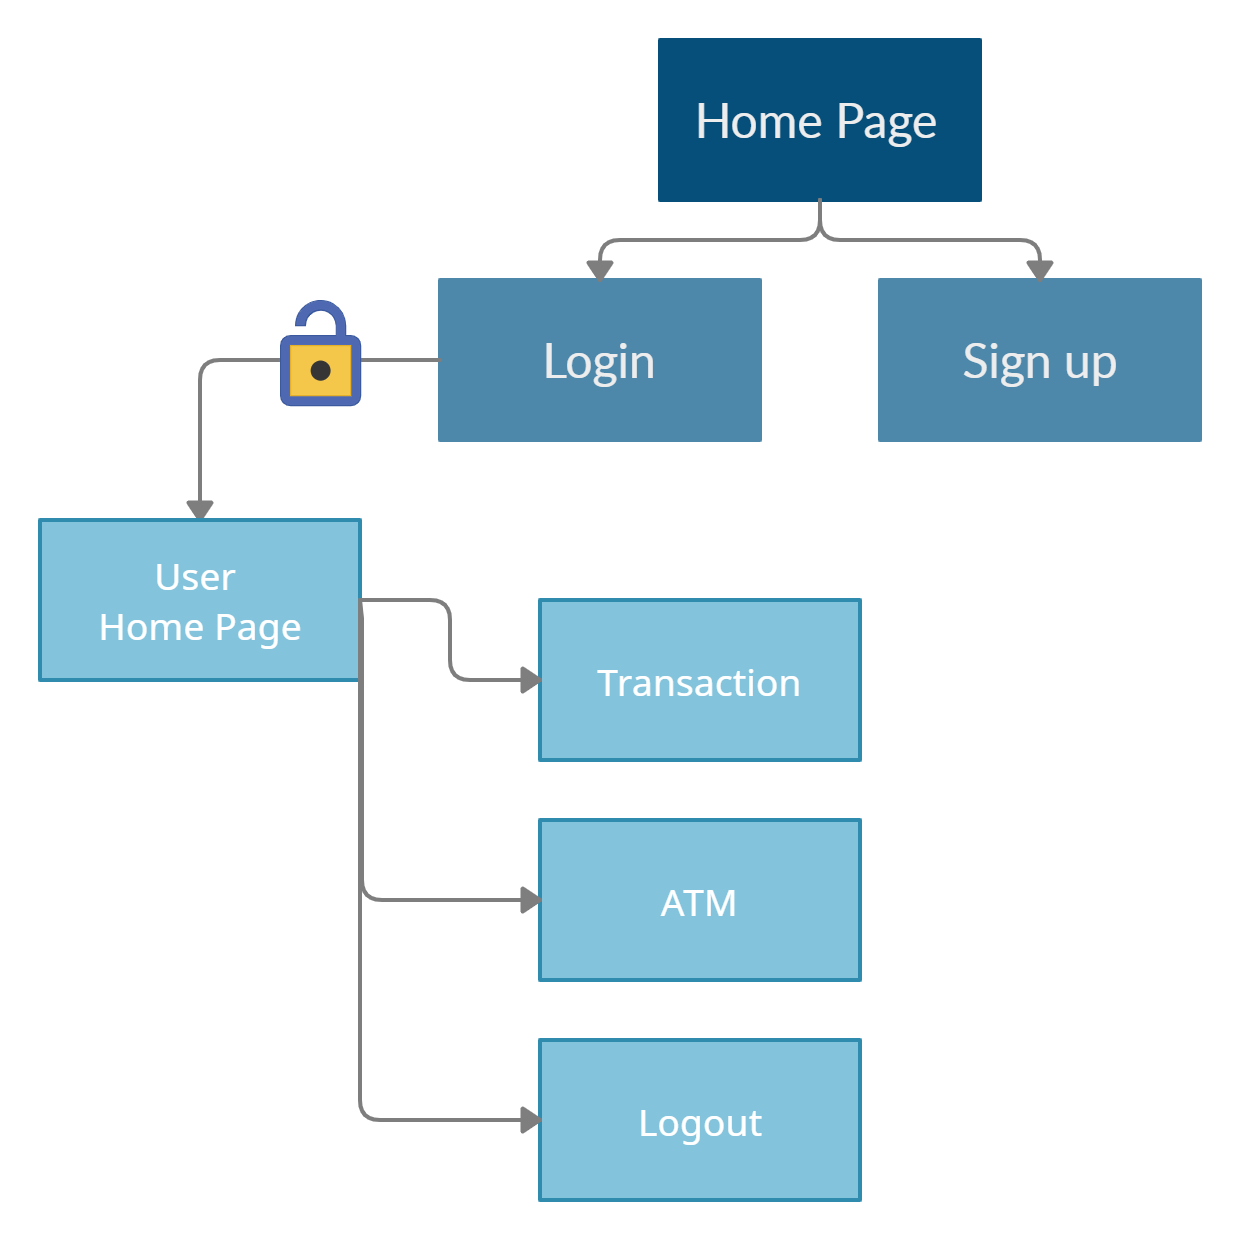
\includegraphics[width=\textwidth]{pics/pic1 Site map.png}
    \caption{Site map}
    \label{fig:kap1fig1sitemap}
\end{figure}

A visitor can only see login and signup pages from the homepage. When an unlogged user tries to visit the URL of any other page, he gets redirected back to the homepage.

\begin{figure}[H]
    \centering
    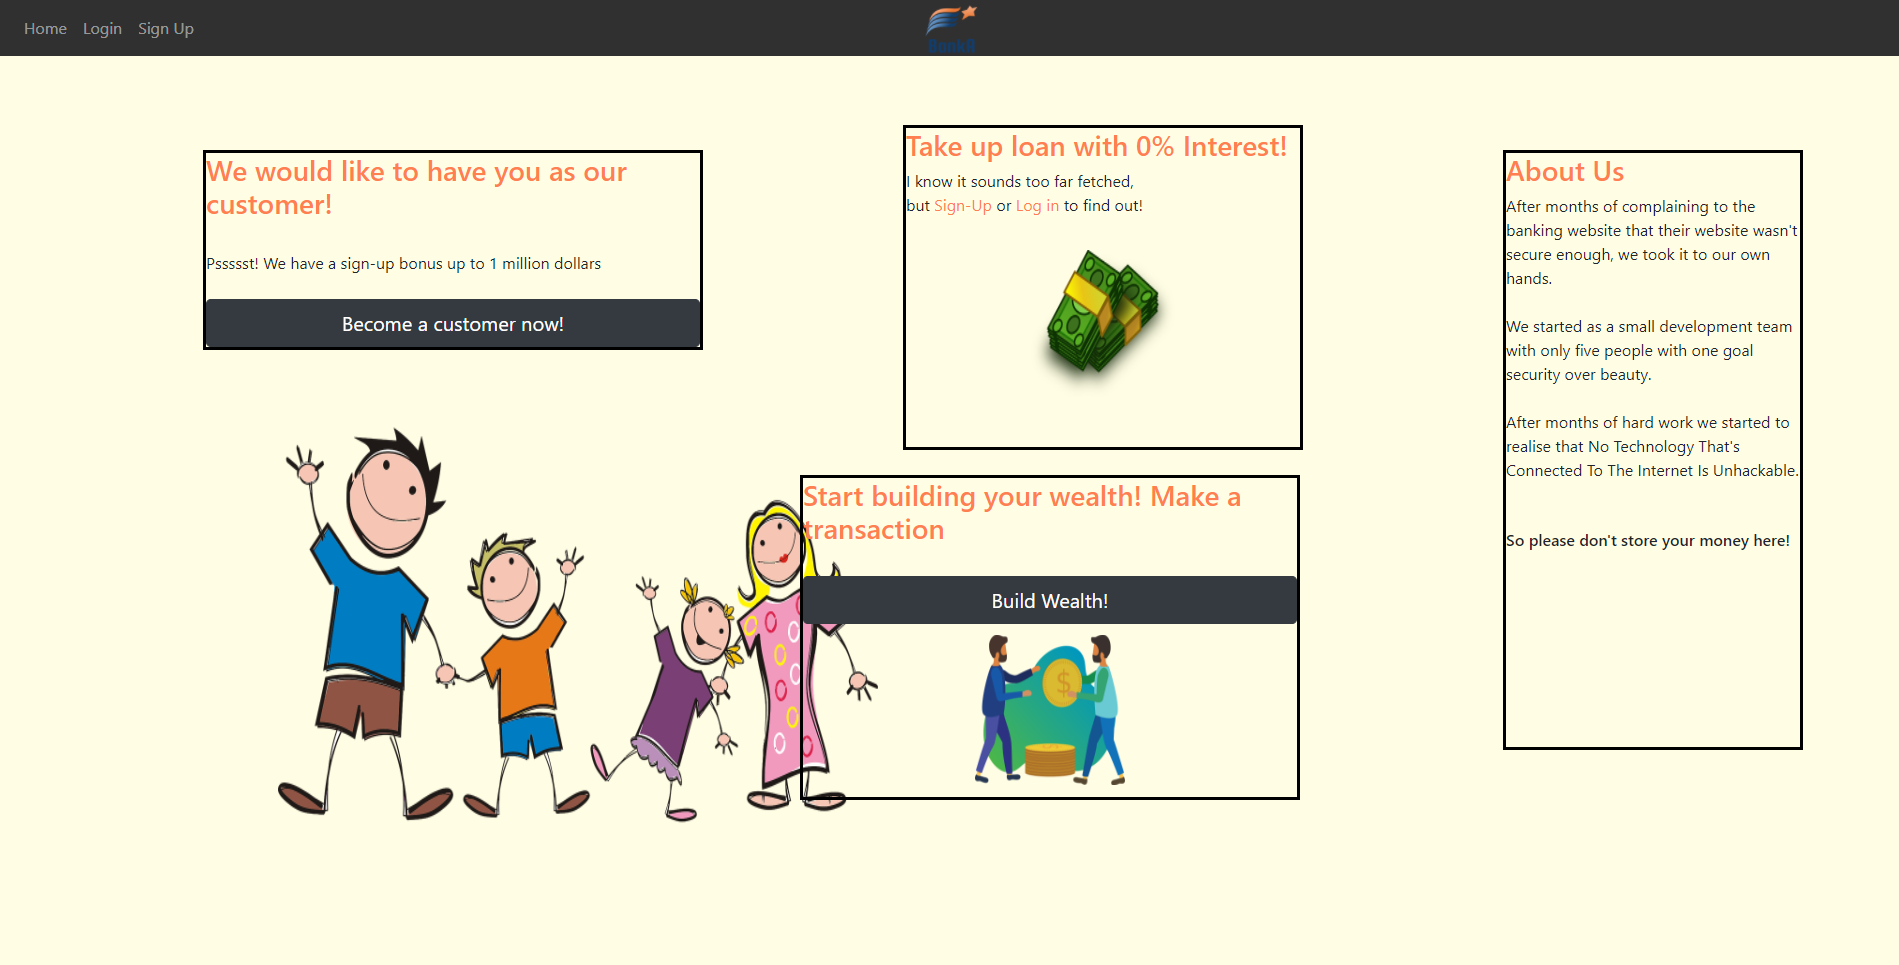
\includegraphics[width=\textwidth]{pics/pic2 home visitor.PNG}
    \caption{Site landing page}
\end{figure}

After logging in, the user gets access to ATM and Transaction pages, also homepage changes to show the user’s balance and transaction history.

\begin{figure}[H]
    \centering
    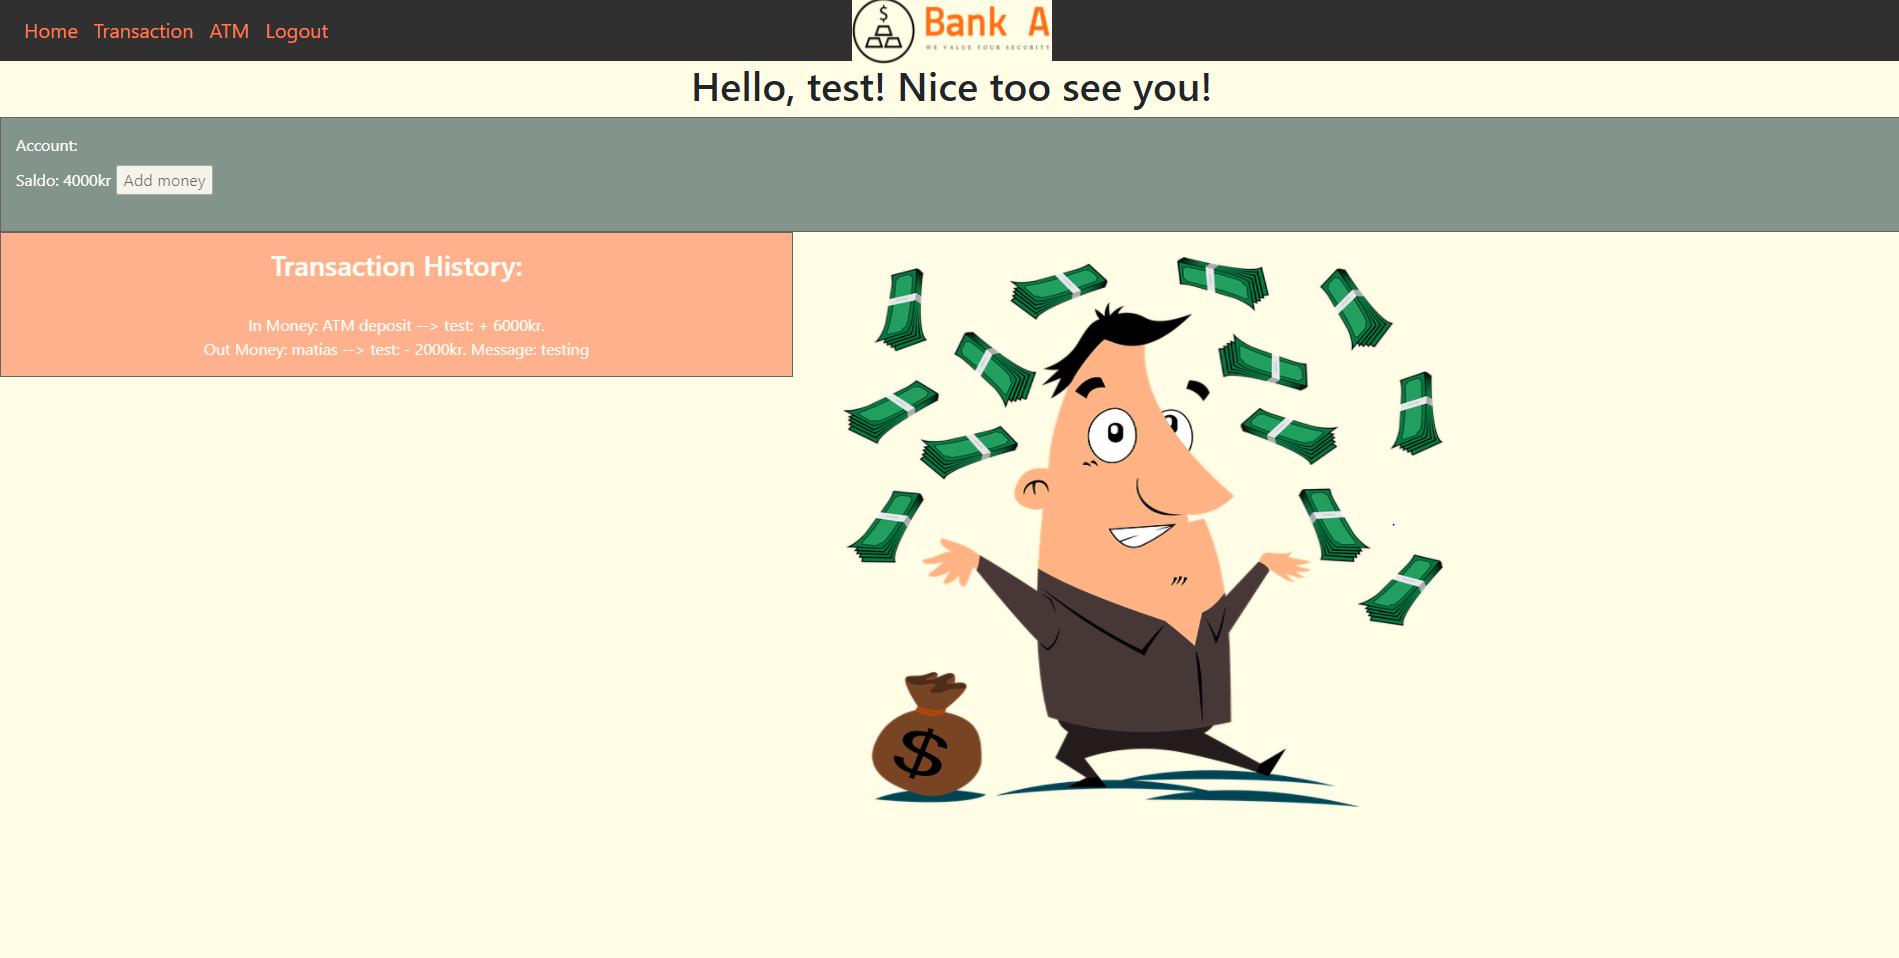
\includegraphics[width=\textwidth]{pics/pic3homeuser.PNG}
    \caption{User homepage}
\end{figure}

\begin{figure}[H]
    \centering
    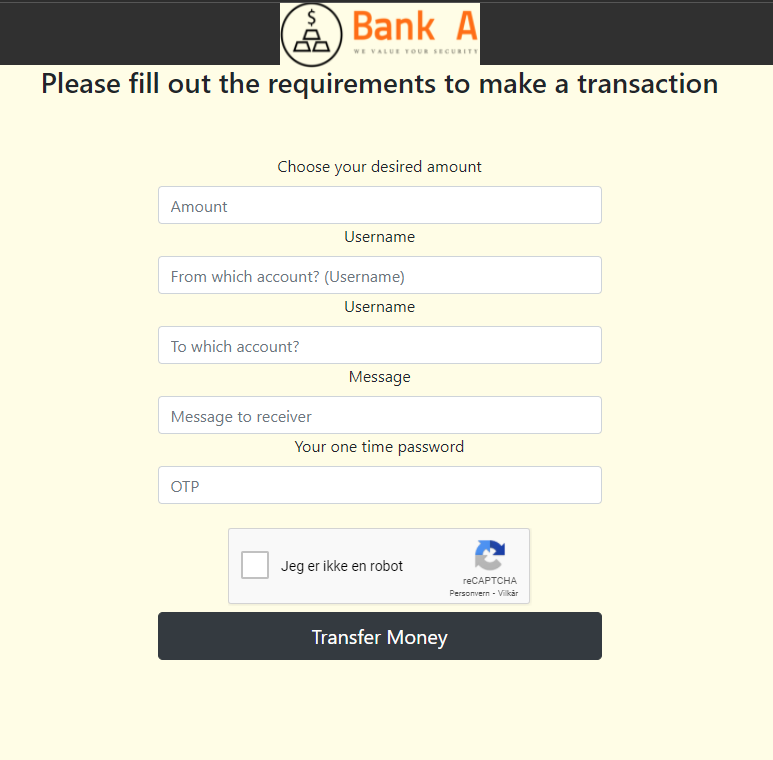
\includegraphics[width=\textwidth]{pics/pic 3.1.PNG}
    \caption{Transaction page}
\end{figure}

To transfer cash from your own bank account in the Transaction page, the user must know the username of the receiver, and in addition confirm his own. The user can also choose to send it with a message. This action must go through reCAPTCHA and 2FA authentication. 

ATM service simulates depositing cash in a local ATM to fill your account. This page looks like this, and must also confirm/verify the name of the user, reCAPTCHA and 2FA authentication. The limit is set to 10 000kr to have realistic values. The ATM page looks like this:

\begin{figure}[H]
    \centering
    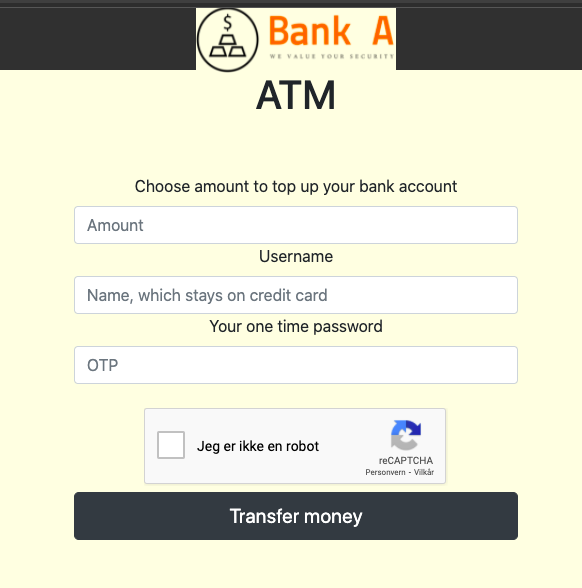
\includegraphics[width=\textwidth]{pics/atmPage.png}
    \caption{ATM page}
\end{figure}

\chapter{Security
}\label{kap:security}

\section{Security and Design}

Here is a data flow diagram to help identify a flow of data and interactions between components in the application:

\begin{figure}[H]
   \centering
   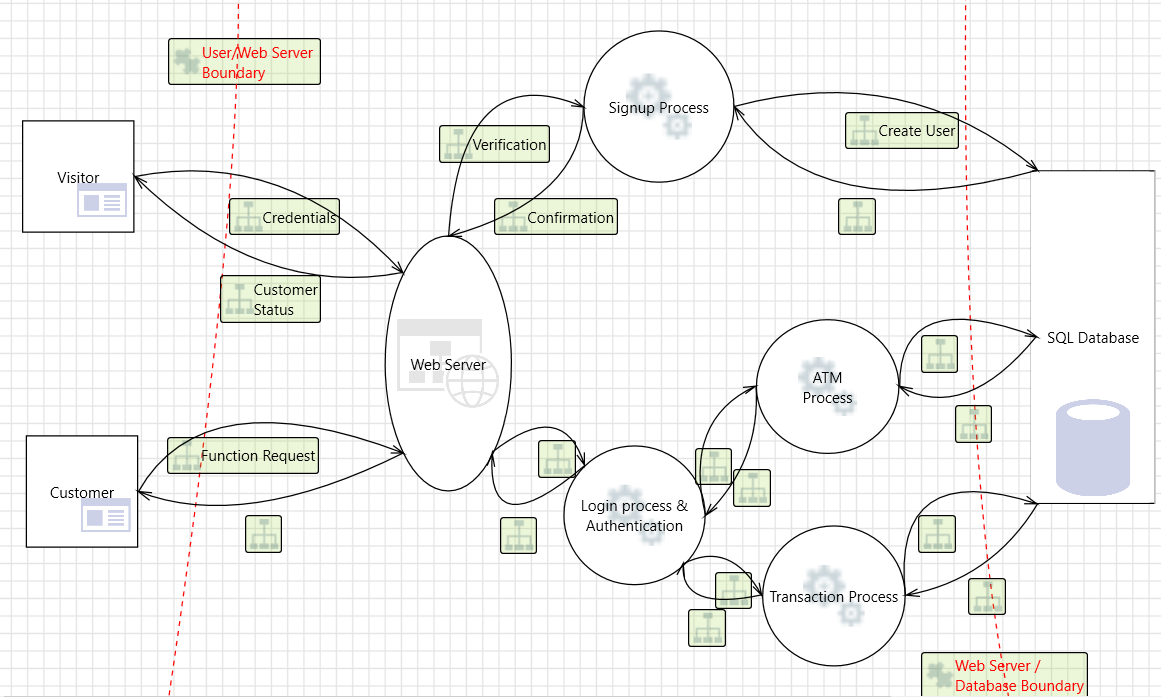
\includegraphics[width=\textwidth]{pics/pic4 Data Flow.PNG}
   \caption{Data flow}
   \label{fig:cha2fig1dataflow}
\end{figure}

Some possible threats that we could identify by looking at the system model are:
\begin{itemize}
   \item Spoofing
   \begin{itemize}
      \item Credential stuffing (attacker having list of valid usernames and passwords)
      \item Brute force authentication
      \item Evading the authentication system and exploiting session management
      \item Cross-Site Request Forgery
      \item Missing session timeouts 
  \end{itemize}
  \item Tampering
  \begin{itemize}
     \item Improper input validation
     \item SQL injection
     \item XML injection
     \item Forcefully browsing to authenticated pages 
     \item tampering with URL to avoid authentication checks
   \end{itemize}
   \item Repudiation
   \begin{itemize}
    \item  Lack of monitoring (performing unauthorized operation without the ability to be traced or detected)
   \end{itemize}
   \item Information disclosure
   \begin{itemize}
     \item Unauthorized access to database
     \item Capturing non-encrypted data
     \item Access to weakly encrypted content
   \end{itemize}
\end{itemize}

In next sections we will show the basics of how our website is structured in the code and how our features are implemented within our website. Lastly we will look at how to mitigate some of these threats mentioned above both in chapter 1 but also in chapter 2. % TODO, ref chapters

\subsection{Design choices}

We “deny by default” all but essential intranet traffic, the only way to have a read/write connection with our database, is to log in, or sign up.
Otherwise, the site is in a "special" read-only status, where you can only view the public html, and get no data from the database. Like most, if not all, secure websites.

We decided that it's better design-wise to have one "master" class for transactions, and not to have a "balance" value in our database table, it comes with a number of advantages:
\begin{itemize}
    \item It's easier to keep track with abnormalities, if anything fishy is going on, our system will show us why and how.
    \item It's much harder to directly change the balance value in the database, since it's not stored in one place, and all the transactions should be read-only once verified and validated.
    \item It's an easier system to manage, than having two separate data classes for normal transaction, and one-user transactions (ATM).
\end{itemize}

\Que{Why can from and out money values be null?}
\Ans{Because ATM process allows for putting in money, where there is not user/user account to get money from}
\Que{Why are we saving money value data in a string?}
\Ans{With some research, there were two options of saving money amounts. Either with a non-fixed point decimal, or a long string. Since SQL\textunderscore Alchemy doesn't support decimals too well.We decided to go with a very long string instead, that way we can have perfect precision, and support very large numbers as well.}

\section{How features are implemented}

\subsection{Getting user input}

WTForms extension is used to gather and validate input from users. Depending on the need, built-in or custom validators are used, unfortunately it can be easily bypassed so this is our front-end checks. We implemented it by  creating a Flask form class which is shown in picture X and this method is used for every input we get from a user. For example, sign-up transactions8 etc. 

\begin{python}
class LoginForm(FlaskForm):
   email = StringField(label='Email', validators=[Email()])
   password = PasswordField(label='Password',
                            validators=[DataRequired(),
                            Length(min=1, max=100,
                            message="Password must be between"
                           +"7 and 100 characters!")])
   
   OTP = IntegerField(label="Your one time password",
                      validators=[DataRequired()])

   recaptcha = RecaptchaField()

   submit = SubmitField(label='Log in')
\end{python}

We validate the user input on our back-end as well using various function to check if it contains any illegal characters. More on this in chapter 4.  %TODO REF

\subsection{Creating user}

When the signup form is sent, the input is validated both within WTforms and on backend, then a check is made to see if a user with a given name or email already exists. If not - then the given password is hashed and user data is sent to the database and saved. The application then redirects you to the homepage. We also logs this info in our log database model. If something goes wrong during the process, a red error message will appear.

\begin{figure}[H]
    \centering
    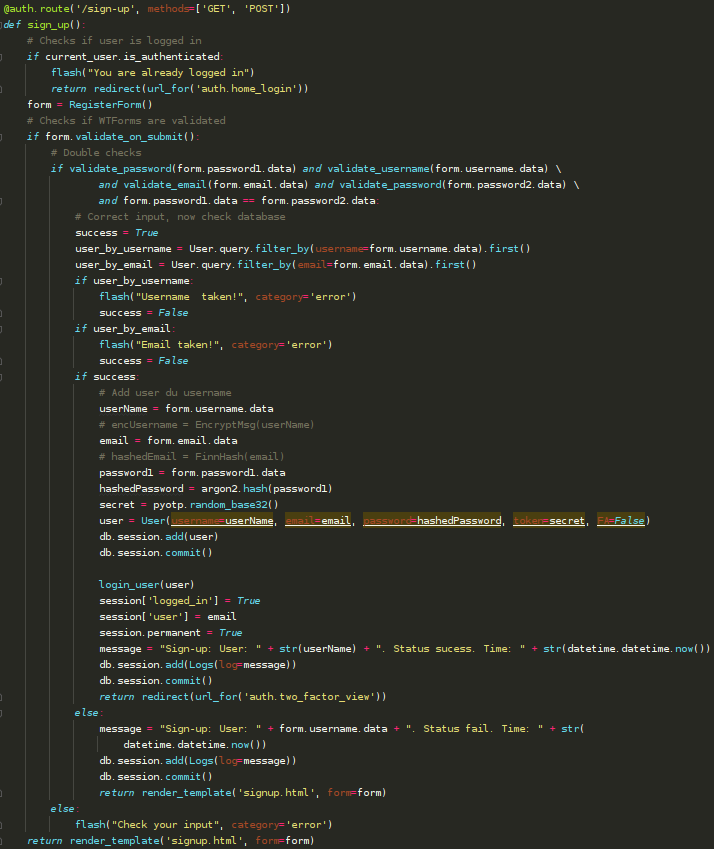
\includegraphics[width=\textwidth]{pics/pic7 signup.png}
    \caption{Sign up backend code}
    \label{fig:cha2fig2signupcode}
\end{figure}

Argon2 function is being used to hash passwords.

\subsection{Login process/Session management}

When the login form is sent, the input is also validated both front-end and backend. Then the database is searched for a user with a given email and given password is compared with hashed database password. It also checks for reCAPTCHA and the OTP (one-time-password) is correct. If everything is okay, the app redirects the user to his homepage. If something goes wrong during the process, a red error message will appear.

\begin{figure}[H]
    \centering
    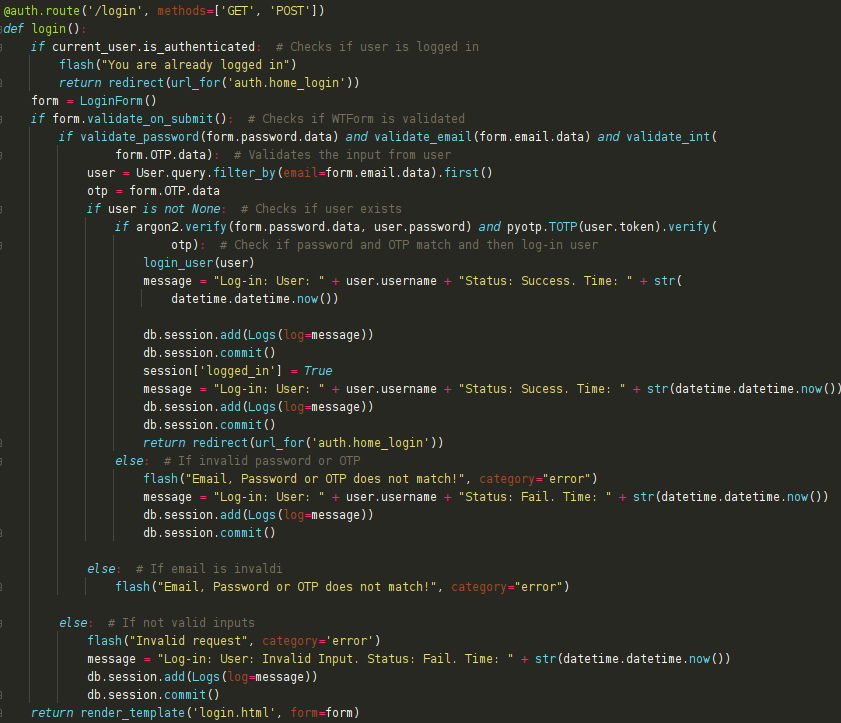
\includegraphics[width=\textwidth]{pics/pic8 login.png}
    \caption{Login backend code}
    \label{fig:cha2fig3logincode}
\end{figure}

Furthermore a user can log out simply by clicking on the logout button in the navigation bar, and gets redirected to the log-in page. 

The application uses the Flask-Login extension for session management. It allows us to restrict some pages to be visible only for logged-in users, but we will go deeper into the security of this in chapter 4. %TODO REF

\begin{figure}[H]
   \centering
   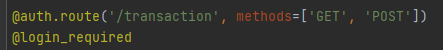
\includegraphics[width=\textwidth]{pics/pic9.1 loginrequired.PNG}
   \caption{Login required}
   \label{fig:cha2fig3loginrequired}
\end{figure}

\begin{figure}[H]
   \centering
   
\includegraphics[width=\textwidth]{pics/pic9.2 need to log in.PNG}
   \caption{No access}
   \label{fig:cha2fig4noaccess}
\end{figure}

\subsection{ATM and Transaction}

These services first validate data both front-end and back-end. Then authenticate given data to check if said username exists, valid amount etc. It also check for reCAPTCHA and OTP. If everything checks out, a transaction is made. If something goes wrong during the process, a red error message will appear. 

\subsection{Database}

Flask-sqlalchemy extension provides support for SQLALchemy. We use three database models – user, transaction and Logs. The user stores the user information, like username, email, password, id, token(used for 2FA) and FA check (whether they have already accesses QR-code page). The password is stores in the database using argon2 hash. We will discuss our approach on why we chose this algorithm in chapter 4. 

In our transaction model we save the id of the transaction, from\_user, to\_user, in and out money and a message. As you have seen we don’t store the account balance in the database as a security measures and to get as close to the real world as possible. We simply use a for loop to go through each transaction for that given user. The implementation looks like this:

\begin{python}
class Transaction(UserMixin, db.Model):
   transaction_id = db.Column(db.Integer, primary_key=True)
   from_user_id = db.Column(db.Text, nullable=True)  
   out_money = db.Column(db.Text, nullable=True)
   to_user_id = db.Column(db.Text) 
   in_money = db.Column(db.Text)
   message = db.Column(db.String(120))
\end{python}

Lastly we have another database model called logs. This simply stores the id of the log and the log message, which contains the action made, user (if any), success or fail and what time it was logged/happened. We store both success made by a user and failures. 

\begin{python}
class Logs(db.Model):
    log_id = db.Column(db.Integer, primary_key=True)
    log = db.Column(db.Text)
\end{python}

\chapter{OWASP Top Ten
}\label{kap:owasptopten}

This section describes how prepared are we against common threats listed in OWASP Top 10 //TODO

%TODO SORT ME prob A1-10

\section{A01 Broken Access Control}

The number one of security breaches is Broken Access Control and therefore very important for our development team. This breach is about being able to acts outside of their intendent permissions. For example if a user is not logged in it can’t view pages on the website that they are not authorized to see or make requests. 

A way to mitigate this flaw is by using flask-login. When a user login we use the login(user) code. This logs the user inn and can access routes in our website that requires a user to log-in. We use the “@login required” parameter for the implemented route. The code makes it so that the user that tries to access the page/route must be logged in. When a user logs out we call the code logout(user). This removes the flag that the user is logged in and has now not access to the pages it had when logged in. The code snippets below demonstrate this. 

Lastly to mitigate this security fault is checking if the user has been inactive for more than 5 minutes. This is important if a user forgets to exit the website or logging out, because then the session cookie will still be available. The implementation looks like this:

\begin{python}
@auth.before_request
def before_request():
    """Timeout user when inactive in 5 min"""
    flask.session.permanent = True
    current_app.permanent_session_lifetime\
        = datetime.timedelta(minutes=5)
    flask.session.modified = True
    flask.g.user = flask_login.current_user
\end{python}

\section{A02 Cryptographic Failures}
Cryptography is the process of turning data into a format that is impossible for humans to extract any information out of. It is especially important when storing private information about people like, credit card number, health records, personal information, etc, in our databases. That also applies to our website where we will store user passwords, transactions, and money.
\subsection{Hash functions}
There are two methods of cryptography that we have employed, the first one is hashing. Hashing turns data into an unreadable mess and has no inverse function to "unhash" that data again. That is a key property that we need for storing sensitive data like passwords which we will never need to display. The hash will always have the same size output no matter what the size of the input, making it harder to reverse-engineer the original string. In the case of passwords we have to make sure that different passwords don't get the same hash, to achieve this hash functions use salts, strings of random characters appended onto the original string to create a unique hash every time. 

The hash function we have decided to use for hashing passwords in our database is argon2-cffi. For password hashing it is important that it is very costly, this is to reduce the time needed to crack the original. Argon2 not only makes hashing passwords costly on the execution time but also on the memory cost and employs parallelism to use several threads. All this combined makes up for an excellent hashing algorithm for passwords.

To implement argon2 in flask we import and use the hash module from passlib:
\begin{python}
from passlib.hash import argon2
\end{python}
The argon2 function has methods for hashing and verifying the hash as following:
\begin{python}
argon2.hash(inputPass)
argon2.verify(hashedPass, inputPass)
\end{python}

The hash method for argon2 takes in a user input password and optional parameters then hashes the password accordingly. The parameters are memory usage, time usage (iterations), and degree of parallelism, which we can call, M, T and P respectively. By default argon2.hash() will have the values: M = 100MB, T = 2 iterations and P = 8 degrees. These values are sufficient to fulfill OWASP's minimum requirement of M=15MiB, T=2 iterations and P = 1 degrees. 

In the code we achieve this by doing:

\begin{python}
password1 = form.password1.data
hashedPassword = argon2.hash(password1)
secret = pyotp.random_base32()
user = User(username=userName,email=email,
    password=hashedPassword,token=secret, FA=False)
db.session.add(user)
db.session.commit()
\end{python}

Here the user input password while signing up will be hashed using argon2 hash function and put into a user class with all the relevant parameters. This class will then be put into the database and committed to be stored there. It is important for the password to be hashed before storing, or else it will be vulnerable to attackers that have gained some form of access to the database. Hashing makes sure that even if the data is breached, it will not be easily decoded. 

\pagebreak
In the case of logging in using that password we use the verify method from argon2. This will return a boolean value if the input password matches the hashed password that is stored in the database. We do this in python with an if-statement: 
\begin{python}
if user is not None and argon2.verify(form.password.data, 
            user.password) and pyotp.TOTP(user.token).verify(otp):
    login_user(user)
\end{python}

This piece of code checks first and foremost that the user actually has an entry in the database, and then if the password given matches that users hashed password. The part with pyotp is for Two-Factor Authentication which is outside the scope of this section. When the code successfully verifies the users password it will then proceed to log the user in and allow them access to all of our services that require it.

\subsection{Encryption}
We use a python package called talisman, it forces the entire website to be ran in https, encrypted http, over TLS or SSL.
So basically an added encryption layer of SSL or TLS. It protects data from eavesdropping and man-in-the-middle attacks.

The other way to utilise cryptography is encryption. The biggest difference between encryption and hashing is that encryption is reversible. That means for every encrypted piece of data, we have a inverse method, which we call decryption to turn it back into readable data. A simple way to assure authenticity is by using keys. The key is a piece of data that will allow you access to encrypt or decrypt the data. Within encryption there are two popular methods to use, symmetric and asymmetric encryption. The former uses the same encryption key for both encryption and decryption, hence the name symmetric, while the latter uses a private key and public key.

For the purposes of our website we have only used symmetric encryption. Symmetric encryption requires the that both the encryption and decryption needs the same key. This brings upon us the challenge of how to securely store the key itself. The recommended and safest way is to use a "Hardware Security Module". This and most other options were not viable or available to us, so due to lack of resources we decided to just let it sit in the source code. This approach is very unsafe, but the only other viable option was storing it in the database, which requires a direct access without going through the code. However seeing as storing it in the database was almost as bad of a solution as just having it in the source code, we decided that it was worth the risk. 

With this naive approach we have decided only encrypt transactions made by users. This way if attackers somehow got access to the database dumps they would be unable to see how much money was transferred without the encryption key. We achieved this in python by using the Fernet module from the crypgraphy import like so:
\begin{python}[language=Python]
from cryptography.fernet import Fernet
\end{python}

This module allows us to use some useful methods to create a function to encrypt and decrypt messages. To do this we first have to initialize our encrypter with the encryption key as following:
\begin{python}
encKey = b'FtSL3pqkp2yHZIDPCmP3e_70WJX2GK2iFpEtPcx7MAk='
Encrypter = Fernet(encKey)
\end{python}

The encryption key encKey was generated using the generate\_key() method from the Fernet module, due to the uncertainty of key generation we have decided to extract it and keep it static for all our purposes. As said before this is very naive and should be avoided if possible. With the encrypter initialized we can create the functions for encryption and decryption:
\begin{python}
def EncryptMsg(string):
try:
    encoded = string.encode()
    encMsg = Encrypter.encrypt(encoded)
except AttributeError:
    nyString = str(string)
    nyEncoded = nyString.encode()
    encMsg = Encrypter.encrypt(nyEncoded)
return encMsg
\end{python}

This function takes in a input and attemts to encode it to bytes. This is because the encrypt method in our encrypter only accepts data in the byte datatype. Python's inbuilt encode() method allows us to turn strings to bytes directly. However encode() only works for strings, hence we have our exception where if the input is anything else, it will attempt to turn it into a string first. This is important for transactions where we want to encrypt the amount. All of this will return a encrypted message which can safely be stored in the database. To decrypt the messages we have made a function for decryption:

\begin{python}
def DecryptMsg(encString):
decMsg = Encrypter.decrypt(encString)
decoded = decMsg.decode()
return decoded
\end{python}

This function is admittedly more simple as it only takes in a encrypted message, uses the decrypt method from our encrypter which will return a byte, then decodes it back to a string object, which we can read as humans. With these functions at our disposal we can use them when we insert and extract from the database. In the following example we will insert the transaction amount as encrypted data:
\begin{python}
new_transaction = Transaction(out_money=EncryptMsg(amount), 
                from_user_id=from_user_name, to_user_id=to_user_name,
                in_money=EncryptMsg(amount), message=message)
    db.session.add(new_transaction)
    db.session.commit()
\end{python}

In this code we are encryption the amount of money transferred before it gets committed to our database. Because we need to use this value later for calculations we have to decrypt it elsewhere, otherwise using a hash function would be the better choice. This calculation is done to find out the sum of money a user has, instead of using fixed amounts, we add and subtract total transactions for a more accurate calculation of money:

\begin{python}
class Transcaction():
out_money = db.Column(db.String(40), nullable=True)
out_money = db.Column(db.String(40), nullable=True)

def get_out_money_decimal(self):
    if self.out_money is None:
        return 0
    return decimal.Decimal(DecryptMsg(self.out_money))
def get_in_money_decimal(self):
    if self.in_money is None:
        return 0
    return decimal.Decimal(DecryptMsg(self.in_money)) 
\end{python}

\pagebreak
Here we use the decryptMsg function we have made to decrypt our database entries before using them in the methods, get\textunderscore out\textunderscore money\textunderscore decimal and \linebreak get\textunderscore in\textunderscore money\textunderscore decimal. These are the methods that are later used in the transaction calculations. That will ensure that we don't use bytes in calculations but integers, that get turned into a decimal with the decimal.Decimal() function.

Ideally we would have wanted to use this for storing usernames as well, but there were certain walls to overcome. We could not get the matching salts if we wanted to compare a user inputted username to a stored encrypted username. This caused a few issues which we decided was not important enough to solve, as we have no restriction in what the username can be, it should not relate to personal information hence storing it encrypted should not be a priority. 

All in all we have a fine structure in the use of cryptography in our website, the hashing part is far more than necessary for OWASP, but the encryption part is severely lacking. But as we have not employed a basis of using real names and addresses in our website, this should be sufficient. 

\section{A03 Injection}

Injection attack happens when web application receives input which can be interpreted a command or query. One of the most notable injection attacks is SQL injection, which can lead to reading, modifying or deleting database by an attacker. Typically injection attacks happens through form input fields, like those in login form.

To avoid this, user input must be validated before it is sent as a query. In addition we also use SQLAlchemy which automatically quotes special characters like apostrophes in data.

(ref. http://www.rmunn.com/sqlalchemy-tutorial/tutorial.html) % TODO
% TODO rest to be finished by lukas

\section{A04 Insecure Design}

This new category in OWASP Top 10 is about flaws in design and system architecture. Some weaknesses and technical requirements need to be thought about before starting the implementation. An example of that could be risk profiling and resource management. “A house is as strong as its foundation”. 
While creating this application we have researched secure way to design systems and created threat model to help us recognize and evaluate possible vulnerabilities. We have also prepared for some known attack methods and evaluated which external packages will be used based on security. Furthermore everything that has been implemented we focus on security, for example by setting bounds to user input so that it don’t cause buffer overflow, sanitize all inputs of a user and a robust error handler so it doesn’t crash our website. 

\section{A05 Security Misconfiguration}

This security flaw is about misconfiguration of the website, for example available administrative interfaces, not good error handling and still being in debug mode etc.
For example when we are in development face we often use debug mode, which makes it easier to debug error in the website but also it automatically update your code changes (at least in flask). This can be harmful if not reverted back on deployment. This is because an attacker loves to get error messages and can easily understand how your website is flawed and in which way.  This is simply to remember to disable debug mode which is this line of code: <code>
Another thing we need to is have an error handler for flask, so that the attacker won´t really know what error happened if it manages to create one. In our application we simply check for any errors and if detected we flash a red error message and redirects you do the home page. This also acts as a protective layer against crashing the website. The code used is:

\begin{python}
@auth.errorhandler(Exception)
def basic_error(e):
    """Error handler so flashes message
    and redirects user if error occur"""
    flash("Something went wrong", category='error')
    return redirect(url_for('auth.home_login'))
\end{python}

Since we don´t use any administrative access because of the potential of being a security risk, all the admin access must have access to the deployment website and can make changes there, not directly on the website. Therefore all users have the same access when using the website.

\section{A06 Vulnerable and Outdated Components}

This Owasp category is about use of unmaintained or out-of-date components with known vulnerabilities. It may become hard to track all dependencies together with nested dependencies.
To work against this we remove all unused dependencies and we check those which are being used, so we would know when one becomes unmaintained. All dependencies are kept on a list together with version used so the process becomes semi-automated.

\section{A07:2021 Identification and Authentication Failures}

This security fault is known as Broken Authentication, which is about user´s identity is breached with weaknesses with the authentication in our application, for example using automated attacks. We have implemented a few things to mitigate this, as reCAPTCHA, ratelimit , two factor authentication, strong password etc.   

Firstly to avoid brute forcing and automated attacks, reCAPTCHA and ratelimit has a huge impact on this. The way we implanted this is making a reCAPTCHA user on google and verifying this in our flask WTforms. <code> reCAPTCHA = recaptchaField() <code>. It is possible to bypass wtforms validators/reCAPTCHA so we also made a request limiter, which makes a response and blocks out the user, which will reset in a couple of minutes. We have sat the limit to 60 POST/GET request since that should be more than enough for a normal user. Anything more than that we will block it. The code we used to implement this is:

\begin{python}
@auth.app_errorhandler(429)
def ratelimit_handler(e):
    try:
        message = "Request Limit: User: " + current_user.username\
                  + ". Time: " + str(datetime.datetime.now())
    except:
        message = "Request Limit: User: None . Time: "\
                  + str(datetime.datetime.now())
    db.session.add(Logs(log=message))
    db.session.commit()
    logout_user()
    session['logged_in'] = False
    return make_response(
        jsonify(
            error="Ratelimit exceeded %s" % e.description + 
                  ". Our BOT killer detected unusual many request."+
                  "Please slow down or turn of your BOT!")
        , 429
    )
\end{python}

If an attacker manages to get ahold of an users password we uses two factor authentication which is compatible with google authenticator. We uses this verification after each transaction, deposit and when we log-in. This makes the attacker not being able to access that users account without also having access to their google authenticator app. This acts like a second layer to the users security.  The code we used to implement this is <code>
We have also implemented many more features to prevent this type of security breach like same message if failed log in attempt but we won´t cover this since it is not the most important. 


\section{A08 Software and Data Integrity Failures}

This new category in 2021 is about making sure application uses trusted packages from external sources. This is because using modules from insecure sources can lead to injection of malicious code into the system.

External packages used in this application are received via python pip to which only maintainers have access to. It shouldn’t be a problem as long as we don’t make a typo in package name – which can be used in “typosquatting” attack, where attacker uploads a malicious code to python pip with a name similar to another package.

We can also manually verify that it was produced by the publisher by downloading package and checking signature file.

\section{A09 Security Logging and Monitoring Failures}

A09 has been recently more important over the years. This security breach includes not being able to detect or log activity on the website. This includes also securing the log functions so that no malicious attacks can go through this feature. 

In our website we log every major request. This includes log in, sign-up, transactions, ATM deposits and if the user goes over the request limiter and the ratelimit function is called. We log both successes and failures. The way we store the data is in a separate table in the database. We simple store a string of text that is set by the request the user makes. So a typical string will contain the request (log-in/sign-up etc.), username (if exists), failed or passed and then lastly what time it happened. The way we implemented this is: <code>

We also verifies that the input doesn’t contain any illegal character, so the way we log things doesn’t become a security breach, for example injection in to the database. This is because so that it is harder to breach the log and loads of information about users becomes available to the attacker. The code for this check is: 

\begin{python}
def validate_username(username):
    """Checks for valid username (only letters and numbers)"""
    if len(username) < 2 or len(username) > 50:
        flash("Username must be longer than one character,"+
              "and shorter than fifty", category='error')
        return False

    # If only contains small and big letters, and numbers
    if re.search("^[a-zA-Z0-9s]+$", username):
        return True
    flash("Username can only contain letters and numbers",
        category='error')
    return False
\end{python}

Another logging information we have is ReCAPTCHA. As you can see from picture below is that we can see the statistic of the uses of it and if it have detected any unusual activity. It will also send us an email if detected anything unusual. The negativity with this is that reCAPTCHA uses a long time to update. It uses a couple of days usually, therefore we cannot solely trust on this. 

\begin{figure}[H]
    \centering
    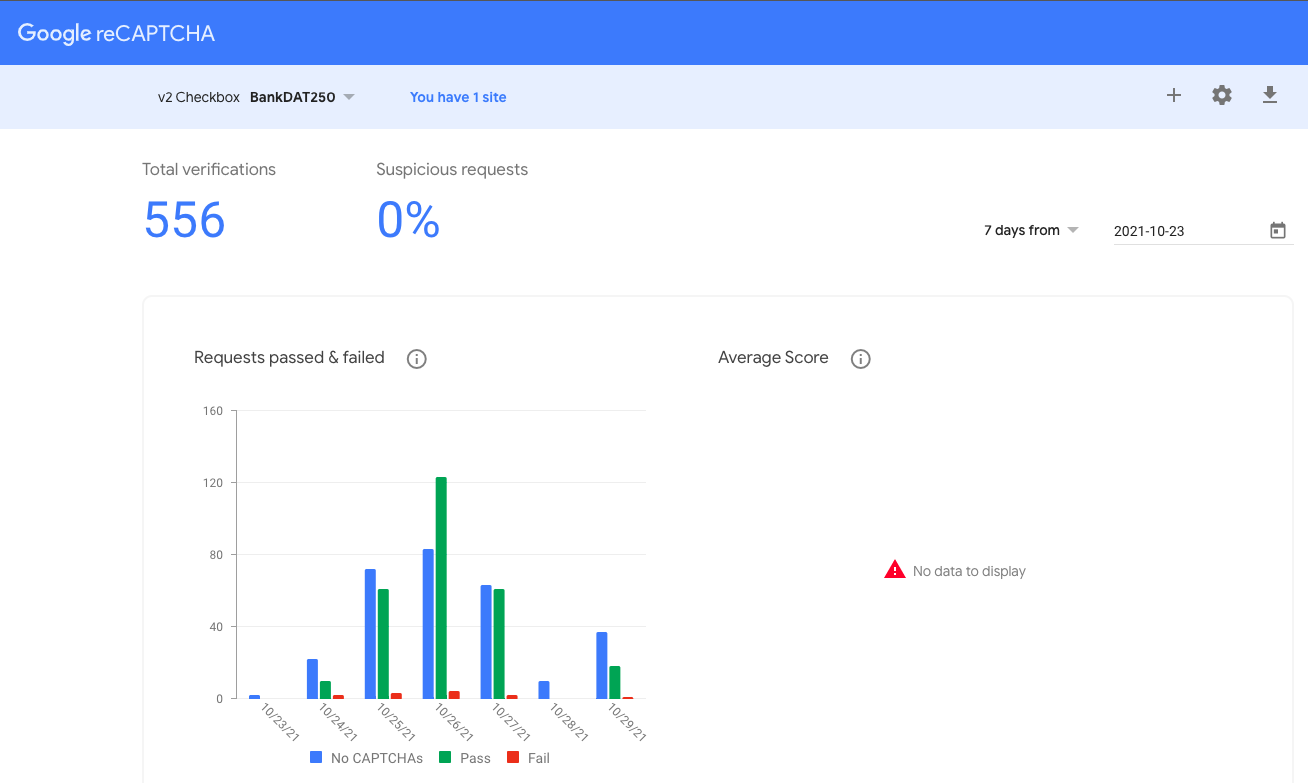
\includegraphics[width=\textwidth]{pics/recaptchaLog.png}
    \caption{reCAPTCHA Log}
    \label{fig:cha3fig1recaptchalog}
\end{figure}

%\input{konklusjon.tex}


% Første linje er bibliografistilen, her finner flere varianter som du
% prøve. Andre linje er selve filen med dine referanser. Siste linje
% legger bibliografi inn i innholdsfortegnelsen. 

%\bibliographystyle{plain}
%\bibliography{referanser.bib}
%\addcontentsline{toc}{chapter}{Bibliografi} 

\appendix

\end{document}


